\subsection{Scratch, Snap! und DataSnap}
\subsubsection{Scratch}
Scratch ist eine visuelle Programmierumgebung, in der Nutzer:innen spielerisch Programmieren erlernen können, indem sie interaktive, visuelle Projekte erstellen. Die Anwendung ist primär an 8- bis 16-jährige Kinder gerichtet \parencite{maloneyScratchProgramming2010}. Grundsätzlich können in Scratch Figuren bewegt werden, welche auf einem Hintergrund (Bühne) angezeigt werden. Durch die definierten Skripte können so beispielsweise Spiele oder animierte Videos erstellt werden.

Abbildung \ref{fig:scratch} zeigt den Scratch-Editor und ein Beispielprogramm. Die Ansicht kann in 3 Spalten unterteilt werden. Links können die Blöcke ausgewählt werden, die in der Mitte zusammengesetzt werden sollen. Der rechte Abschnitt ist unterteilt, in einen Ausgabebereich, und ein Verwaltungsbereich für Figuren und Bühnen. Die Blöcke im Auswahlmenü sind thematisch sortiert. Die Farbgebung spiegelt dies wieder (Vgl. Abbildung \ref{fig:scratch-types}). Um Blöcke im Skriptbereich zu verwenden, müssen sie mittels \textit{Drag and Drop} nach rechts gezogen werden. Skripte sind an Figuren gebunden. Im Beispielprogramm wird die Tiger-Figur nach Start des Programms bewegt und rotiert, sobald die Leertaste gedrückt wird.
\parencite{maloneyScratchProgramming2010}

\begin{figure}[!ht]
  \begin{center}
    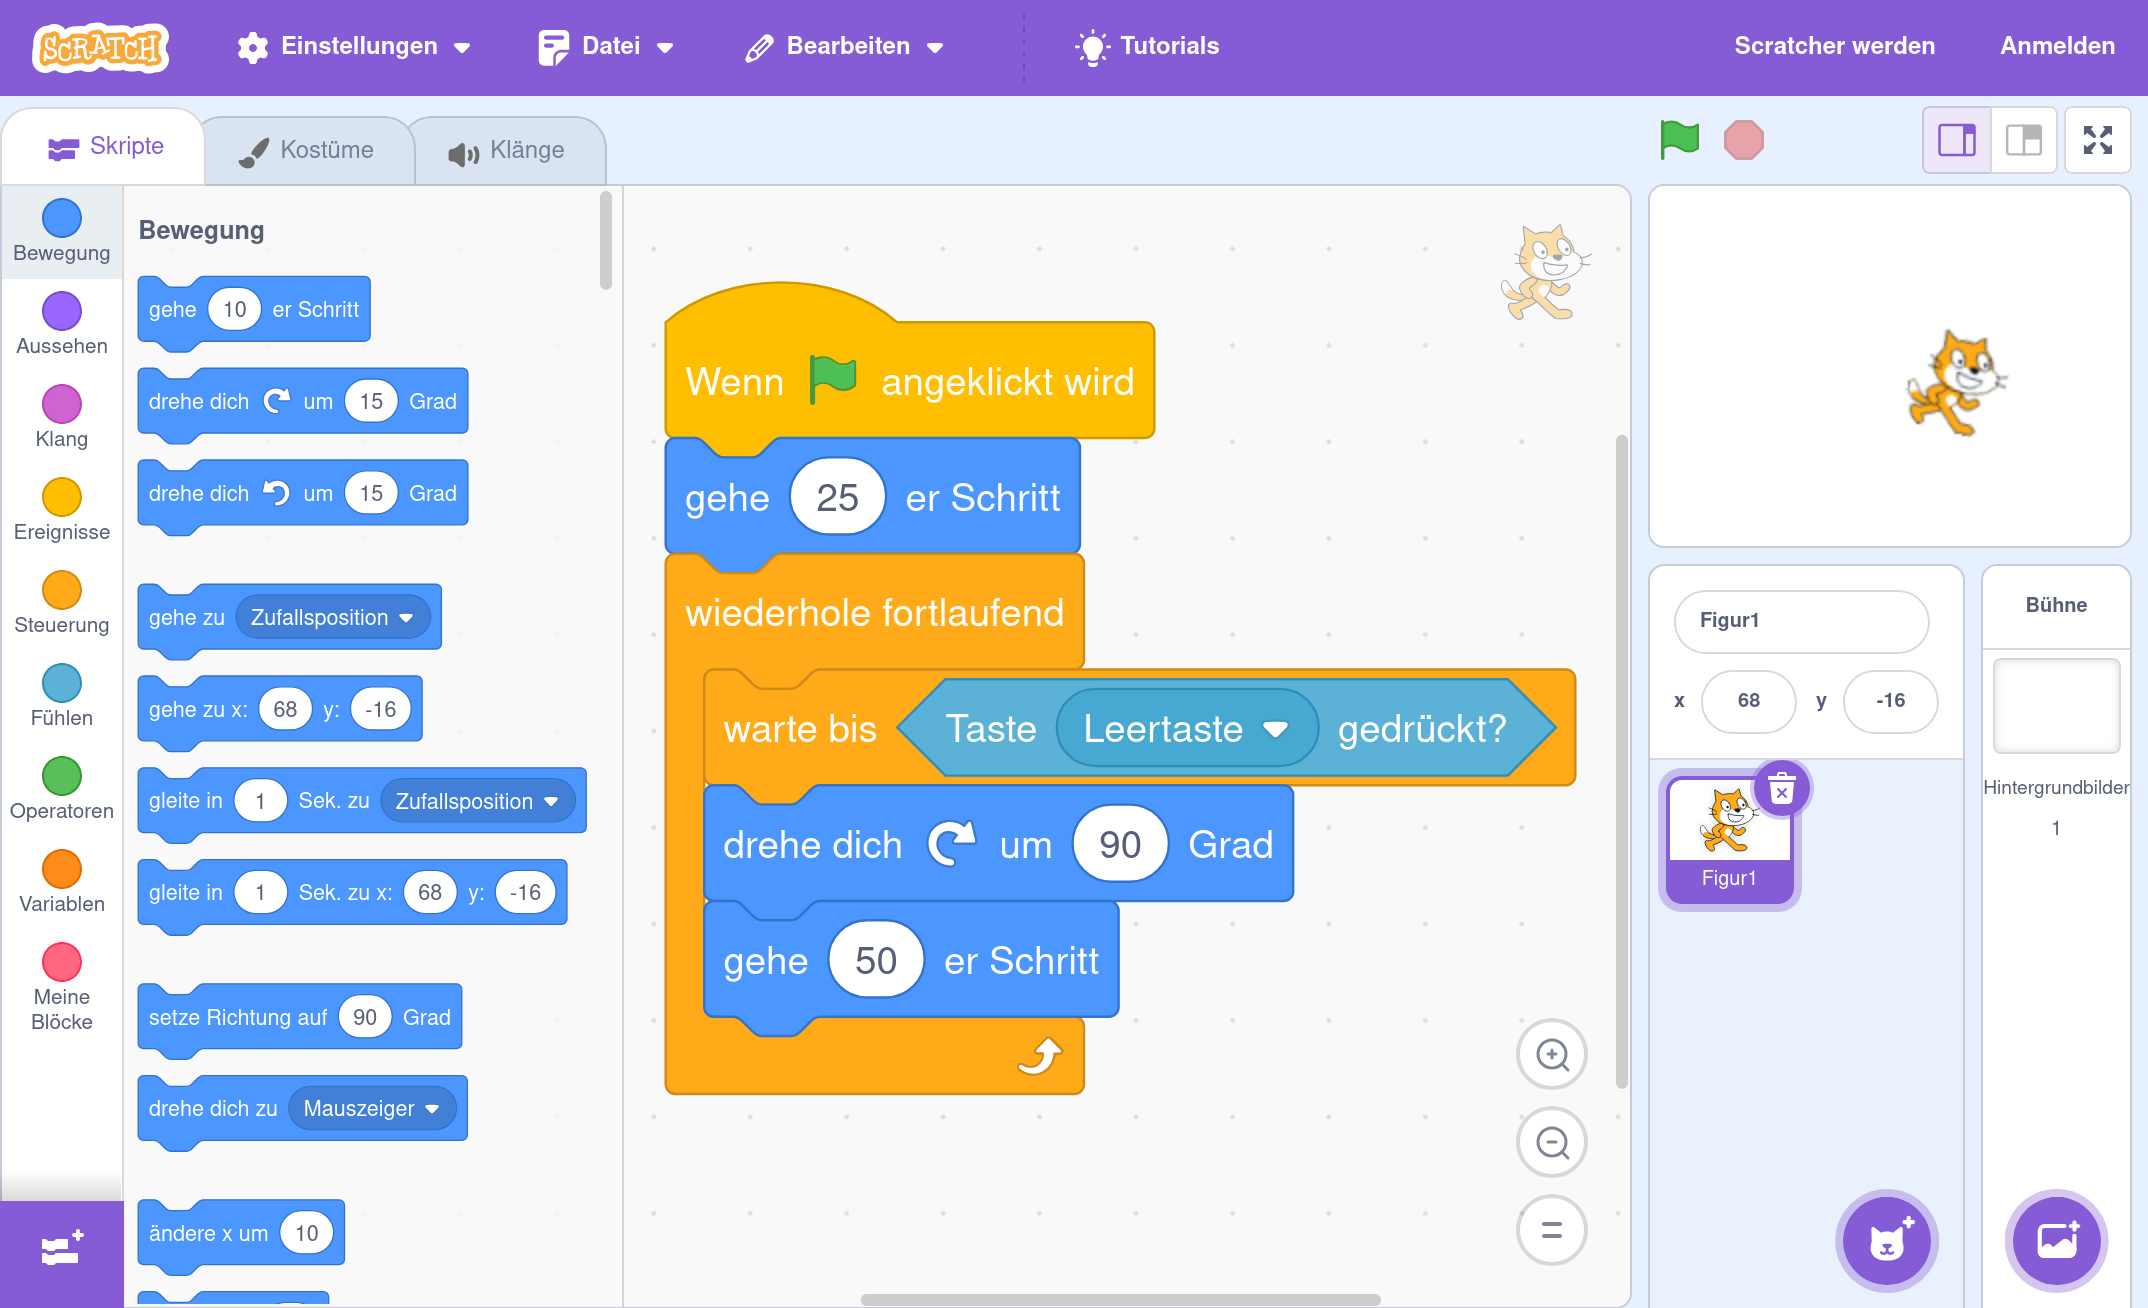
\includegraphics[width=0.95\textwidth]{assets/scratch.png}
  \end{center}
  \caption{Beispielprogramm in Scratch. \parencite{scratchfoundationScratch}}
  \label{fig:scratch}
\end{figure}

Scratch definiert grundsätzlich vier Blockformen \parencite{maloneyScratchProgramming2010}. In Abbildung \ref{fig:scratch-blocks} werden sie verglichen. \textbf{Befehle} führen Programmlogik aus, die beispielsweise Figuren bewegen oder Variablen anpassen. Sie besitzen typischerweise eine Kerbe am oberen Rand und Verbindungsstelle am unteren Rand. \textbf{Funktionen} geben Werte zurück, die errechnet werden können oder in Variablen gespeichert wurden. Es ist nicht möglich, Funktionen an Blöcke mit Kerben anzufügen, sie können aber in korrespondierende Felder innerhalb von Blöcken eingesetzt werden. \textbf{Auslöser} besitzen keine Kerbe am oberen Rand, und stellen den Anfang der Ausführung des angehängten Konstrukts dar. \textbf{Kontrollstruktur-Blöcke} haben die gleiche Form wie Befehle und können wie sie angewendet werden. Sie beeinflussen den Ablauf des Programms und bilden Programmierkonzepte wie Schleifen und Bedingungen ab. Abbildung \ref{fig:scratch} zeigt eine "wiederhole fortlaufend"-Schleife. Es ist zu sehen, dass diese Art von Block auch weitere Blöcke annehmen kann, die im Schleifenkörper ausgeführt werden.
\parencite{maloneyScratchProgramming2010}

\begin{figure}
  \begin{center}
    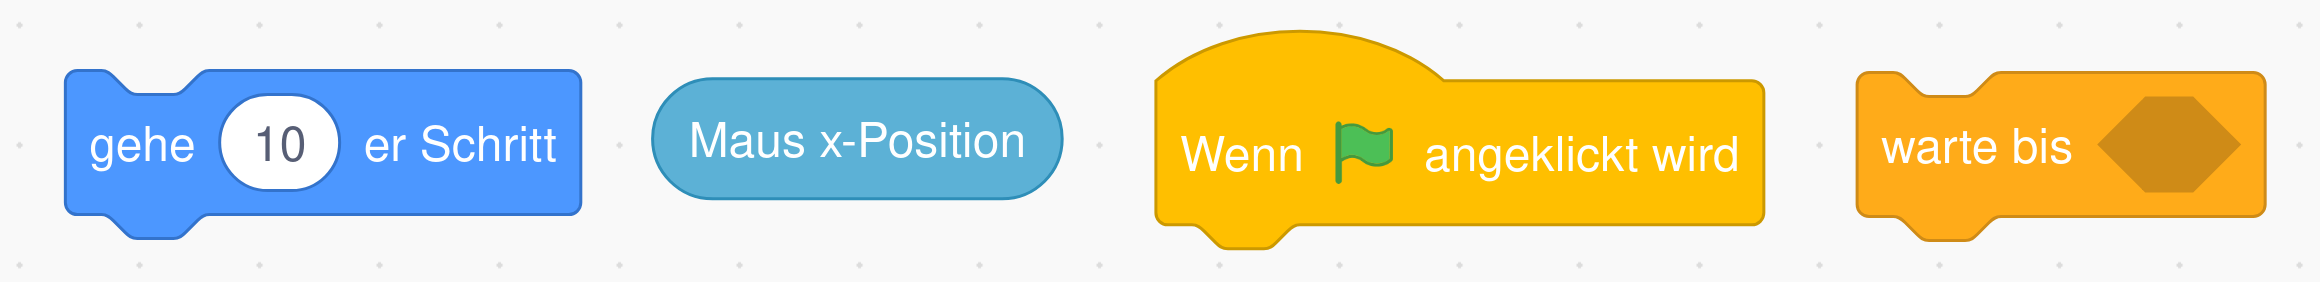
\includegraphics[width=0.95\textwidth]{assets/scratch-blocks.png}
  \end{center}
  \caption{Blockformen in Scratch (v. l. n. r.): Befehl, Funktion, Auslöser, Kontrollstruktur. \parencite{scratchfoundationScratch}}
  \label{fig:scratch-blocks}
\end{figure}

Die Programmiersprache Scratch beschränkte sich zunächst auf drei Datentypen \parencite{maloneyScratchProgramming2010}. Dabei handelt es sich um Text, Zahl und Wahrheitswerte. Texte und Zahlen werden mit abgerundeten Ecken dargestellt, während Wahrheitswerte spitze Ecken besitzen. In Abbildung \ref{fig:scratch-types} werden zwei Funktionen mit unterschiedlichen Datentypen gezeigt, sowie Blöcke die diese als Eingabewerte entgegennehmen können. In den blauen und lila-farbigen Blöcken können auch manuell Werte eingegeben werden, der blaue Block nimmt jedoch nur Zahlen an. Die Datentypen in Scratch wurden mit Nachfolgeversionen erweitert, Version 1.3 führte beispielsweise Listen ein \parencite{harveyBringingNo2010}.

\begin{figure}[!ht]
  \minipage[t]{.49\textwidth}
  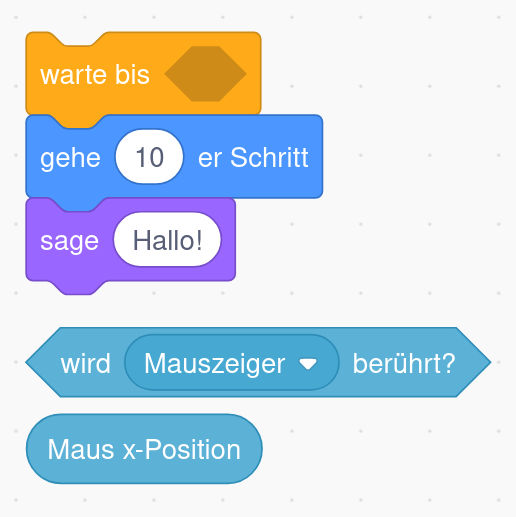
\includegraphics[width=\linewidth]{assets/scratch-types.png}
  \caption{Drei der Blockkategorien in Scratch: Steuerung (Orange), Bewegung (Blau), Aussehen (Lila). Datentypen in Scratch: Boolean (zugespitzte Blöcke), Zahlen und Text (abgerundete Blöcke). \parencite{scratchfoundationScratch}}
  \label{fig:scratch-types}
  \endminipage
  \hfill
  \minipage[t]{.49\textwidth}
  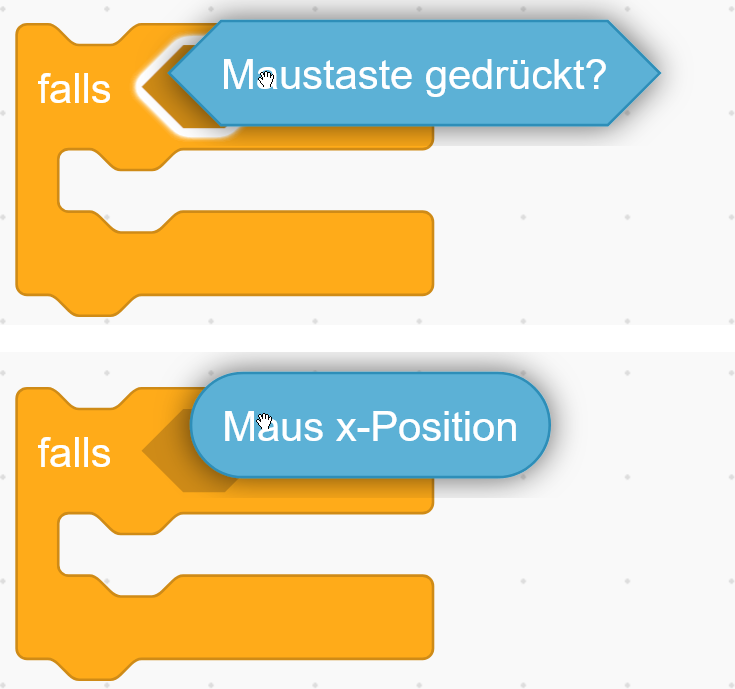
\includegraphics[width=\linewidth]{assets/scratch-drop.png}
  \caption{Blöcke können nur ineinander gesetzt werden, wenn der Datentyp übereinstimmt. Dies wird durch einen weißen Indikator vermittelt. \parencite{scratchfoundationScratch}\todo{ersetzen durch DIY Bild}}
  \label{fig:scratch-drop}
  \endminipage
\end{figure}

Scratch signalisiert über die Form der Blöcke, ob sie zusammengesetzt werden können. Zusätzlich wird beim \textit{Drag and Drop} über einen weißen Indikator gezeigt, ob Blöcke an der aktuellen Stelle eingesetzt werden können. In Abbildung \ref{fig:scratch-drop} ist zu sehen, wie so signalisiert wird, dass eine Wenn-Abfrage nur Wahrheitswerte annehmen kann.

Eine grundlegende Überlegung die bei der Entwicklung von Scratch getroffen wurde, war das Verzichten auf Fehlermeldungen \parencite{maloneyScratchProgramming2010}. Nutzer:innen sollten anhand der Form der Blöcke erkennen, ob es möglich ist, Elemente miteinander zu kombinieren und durch probieren herausfinden, was funktioniert \parencite{maloneyScratchProgramming2010}.

Scratch wird auch im Bildungsbereich genutzt, sowohl im schulischen Bereich \parencite{ortiz-colonTeachingScratch2016}, als auch an Universitäten \parencite{dekerekiScratchApplications2008, harveyBringingNo2010, martinez-valdesRelativelyUnsatisfactory2017}. Der Erfolg dieser Anwendung variiert, führt jedoch oft zu Motivationssteigerungen \parencite{dekerekiScratchApplications2008, martinez-valdesRelativelyUnsatisfactory2017}. Dies ist besonders bei jüngeren Zielgruppen der Fall \parencite{ortiz-colonTeachingScratch2016}.

\subsubsection{Snap}
- \parencite{harveySnapBuild}
- \parencite{harveySnapReference2020}
- \parencite{ballSnapLook2019}
- \parencite{harveyBringingNo2010} (schauen was nicht geht und wie BYOB zu snap führte)
- inspired by scratch
- names: blocks, scripts and sprites erklären
- layout erklären, dabei funktionsweise
- formen um zu zeigen was geht
- drag and drop indicators um zu zeigen dass sachen nicht gehen (reference p. 11)

% \begin{figure}[!ht]
%   \centering
%     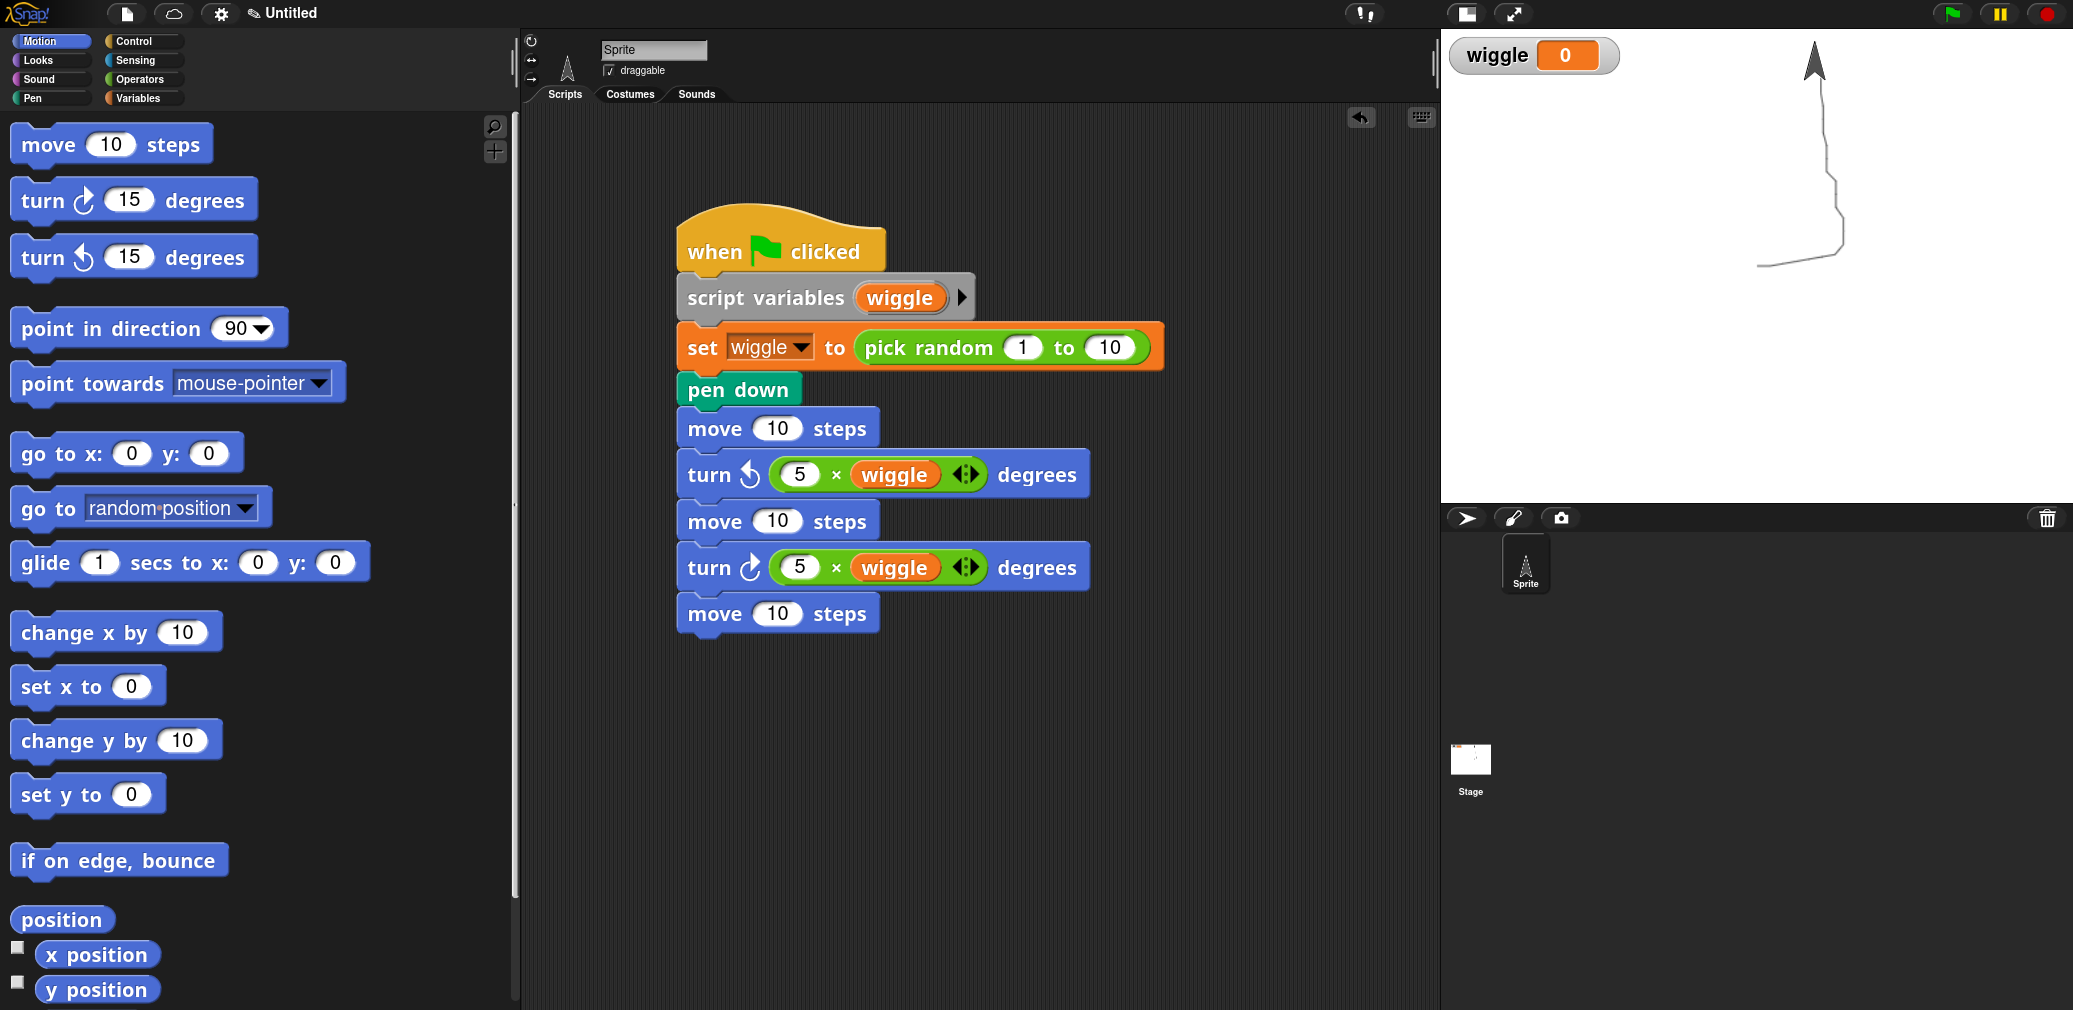
\includegraphics[width=0.95\textwidth]{assets/snap-regions.png}
%   \caption{Regionen im Snap Editor: \textit{Tool Bar}, \textit{Palette}, \textit{Scripting Area}, \textit{Stage}, \textit{Sprite Corral}. Gezeigt ist ein Beispiel aus der Dokumentation. \parencite{harveySnapReference2020}}
%   \label{fig:snap-regions}
% \end{figure}

\subsubsection{DataSnap}
- 4 eigenschaften des papers erklären (p. 19) (und zwei abschnitte oben drüber)
- komplexere Blöcke vordefinieren (p. 26)

- bilder mit blöcken und so (ist das definieren ein snap feature??? - BYOB!)

\begin{figure}[!ht]
  \centering
    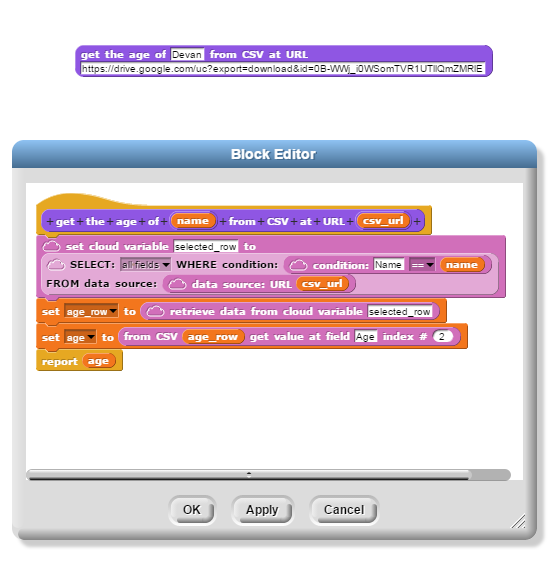
\includegraphics[width=0.95\textwidth]{assets/datasnap-block-definition.png}
  \caption{Anlegen einer Abfrage zur späteren Wiederverwendung. \parencite{hellmannDataSnapEnabling2015}}
  \label{fig:datasnap-block-definition}
\end{figure}

\begin{figure}[!ht]
  \centering
    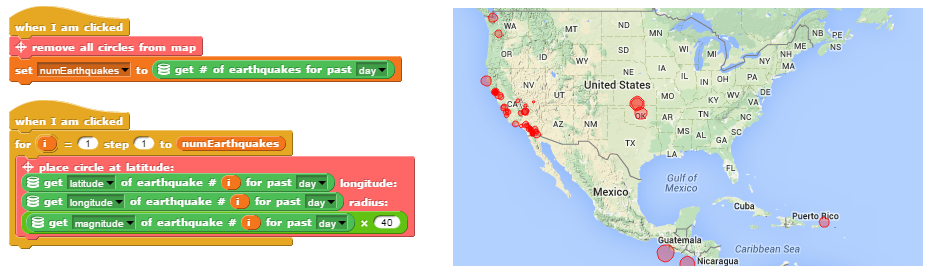
\includegraphics[width=0.95\textwidth]{assets/datasnap-visualization.png}
  \caption{Visualisierung eines Datensatzes über Erdbeben in DataSnap. \parencite{hellmannDataSnapEnabling2015}}
  \label{fig:datasnap-visualization}
\end{figure}

- inwiefern unterscheidet sich datasnap von s4d projekt?


\parencite{hellmannDataSnapEnabling2015} (Chapter 3: DataSnap for Domain Experts)
- based on Snap! 
  - inspired by scratch 
